\documentclass[conference]{IEEEtran}

\usepackage{cite}
\usepackage{graphicx}
\usepackage{amsmath,amssymb,amsfonts}
\usepackage{booktabs}
\usepackage{array}
\usepackage{url}
\usepackage{hyperref}
\usepackage{float}
\usepackage{caption}
\usepackage{subcaption}

\title{Financial Market Prediction Using RNN, LSTM, and GRU Models}

\author{
\IEEEauthorblockN{Sir Asif Ameer, Omer Farooq Khan, Aun Ali, Ahsan Butt}
\IEEEauthorblockA{
Department of Computer Science\\
Your University Name\\
email1@domain.com, email2@domain.com, email3@domain.com, email4@domain.com
}
}

\begin{document}
\maketitle

\begin{abstract}
This project presents a real-time financial market prediction system based on recurrent deep learning architectures. Three sequential models---Simple RNN, LSTM, and GRU---were developed, trained, and evaluated for next-hour market direction prediction using hourly OHLCV data from Yahoo Finance. The system integrates live data ingestion, preprocessing, model inference, and interactive visualization into a unified pipeline. Comparative analysis shows that gated architectures (LSTM and GRU) effectively capture temporal patterns, with GRU providing a strong accuracy-efficiency trade-off. This report documents the complete methodology, experimental results, challenges encountered, and deployment implementation.
\end{abstract}

\begin{IEEEkeywords}
Financial prediction, time-series forecasting, recurrent neural networks, LSTM, GRU, RNN, deep learning, market analytics
\end{IEEEkeywords}

\section{Introduction}
Financial market prediction remains a challenging problem in machine learning due to noisy price signals, non-stationary dynamics, and the influence of global events. Recurrent neural networks (RNNs) are well-suited for time-series problems because they maintain hidden states across sequences, enabling them to learn long-range temporal dependencies.

This project implements a complete real-time market prediction system using three recurrent architectures: Simple RNN, Long Short-Term Memory (LSTM), and Gated Recurrent Unit (GRU). The system continuously fetches hourly market data, applies preprocessing and normalization, and generates next-hour direction predictions. A browser-based dashboard enables real-time model switching and visualization.

The primary objectives are: (1) to build a robust data ingestion and preprocessing pipeline, (2) to train and compare three distinct recurrent architectures, (3) to deploy an interactive web interface for inference, and (4) to provide a detailed technical analysis of model performance and implementation lessons learned.

\section{Authors and Contributors}
The project group members are:
\begin{itemize}
    \item Sir Asif Ameer
    \item Omer Farooq Khan
    \item Aun Ali
    \item Ahsan Butt
\end{itemize}

All members contributed to data collection, preprocessing, model development, evaluation, dashboard implementation, and report preparation.

\section{Methodology}

\subsection{Data Collection Process}
Real-time hourly financial data was collected using the Yahoo Finance API via the yfinance Python library. The collection pipeline retrieves the most recent 7 days of hourly candles including Open, High, Low, Close, and Volume values. The automated fetching ensures that the inference system always operates on the latest available market state, enabling true real-time predictions.

Data validation checks were implemented to handle missing values, network timeouts, and API rate limits gracefully.

\subsection{Preprocessing Steps}
Raw time-series data was transformed into supervised learning samples through the following pipeline:

\begin{enumerate}
    \item \textbf{Chronological Sorting}: Records were sorted by timestamp to maintain temporal order.
    \item \textbf{Invalid Value Removal}: Records with missing or null OHLCV values were excluded.
    \item \textbf{Feature Selection}: Only OHLCV features were retained; other metadata was discarded.
    \item \textbf{Sequence Generation}: Fixed-length sliding windows (lookback=5) were created from consecutive candles.
    \item \textbf{Normalization}: Features were normalized using z-score (mean centering and standard deviation scaling) applied per-window to avoid data leakage.
    \item \textbf{Target Labeling}: The target was set to 1 (up) if the next period's close exceeded the current period's close, and 0 (down) otherwise.
\end{enumerate}

A lookback window of 5 hours was chosen to balance model learning capacity with recent market context. Normalization was performed within each window rather than globally to ensure consistency between training and inference.

\subsection{Model Architecture Explanation}
Three recurrent architectures were implemented in Keras/TensorFlow:

\begin{itemize}
    \item \textbf{Simple RNN}: A baseline recurrent layer with 50 units, dropout regularization (0.2), followed by dense layers. This model serves as a reference for comparing more complex architectures.
    
    \item \textbf{LSTM}: A gated recurrent architecture with 50 units, featuring input, forget, and output gates that enable selective memory retention. LSTM is designed to mitigate vanishing gradient problems and capture long-term dependencies.
    
    \item \textbf{GRU}: A compact gated recurrent unit with 50 units, combining the input and forget gates into a single update gate. GRU typically converges faster than LSTM with fewer parameters.
\end{itemize}

Each model receives a normalized sequence of 5 hourly candles (shape: 5×5) and outputs a single probability value indicating upward movement likelihood.

\subsection{Reasoning Behind Model Selection}
The three architectures were selected to provide a comprehensive comparison across recurrent model complexity:

\begin{itemize}
    \item \textbf{RNN as Baseline}: Simple RNN establishes a foundational performance baseline and helps identify whether added complexity in gated architectures provides real benefit.
    
    \item \textbf{LSTM for Long Dependencies}: LSTM's gating mechanism was chosen to capture complex temporal patterns that may span multiple hours of market activity.
    
    \item \textbf{GRU for Efficiency}: GRU was selected to explore whether a simpler gated architecture can match LSTM performance with faster training and lower memory overhead.
\end{itemize}

This comparative approach is valuable for both academic understanding and practical deployment considerations.

\section{Dataset Overview}

\subsection{Data Sources}
The primary dataset source is Yahoo Finance, accessed via the yfinance API. This source provides reliable, tick-accurate historical and live market data for major financial instruments.

\subsection{Dataset Structure}
Each record in the dataset contains:
\begin{itemize}
    \item Timestamp (datetime, UTC)
    \item Open (opening price)
    \item High (highest price in period)
    \item Low (lowest price in period)
    \item Close (closing price)
    \item Volume (trading volume)
\end{itemize}

The default ticker symbol is SPY (S\&P 500 ETF), which provides broad market representation.

\subsection{Time-Series Description}
This is a supervised binary classification task on time-series data. Training samples are constructed as 5-hour sliding windows with a binary label indicating next-hour price direction. The class distribution is naturally determined by market movement patterns, which may be slightly imbalanced depending on the collection period.

\subsection{Challenges in Data Collection and Preparation}

Several challenges were encountered and addressed:

\begin{itemize}
    \item \textbf{Limited Historical Availability}: Hourly data older than a few years may not be easily accessible, restricting training dataset size.
    
    \item \textbf{Inconsistent Fetching}: Network interruptions and API rate limits occasionally caused data retrieval failures; these were handled with retry logic and error checking.
    
    \item \textbf{Data Freshness}: Ensuring the latest candles are used rather than cached stale data required careful timestamp management and cache invalidation.
    
    \item \textbf{Sequence Alignment}: Matching preprocessed sequences to their corresponding labels required precise index tracking to avoid off-by-one errors.
    
    \item \textbf{Scaling Consistency}: Training data was normalized using parameters computed from training data, while inference data required normalization using the same parameters to avoid distribution mismatch.
\end{itemize}

\section{System Architecture}

\subsection{Data Pipeline Architecture}
Figure~\ref{fig:data_pipeline} illustrates the complete data pipeline from raw market data to model-ready training sequences.

\begin{figure}[H]
    \centering
    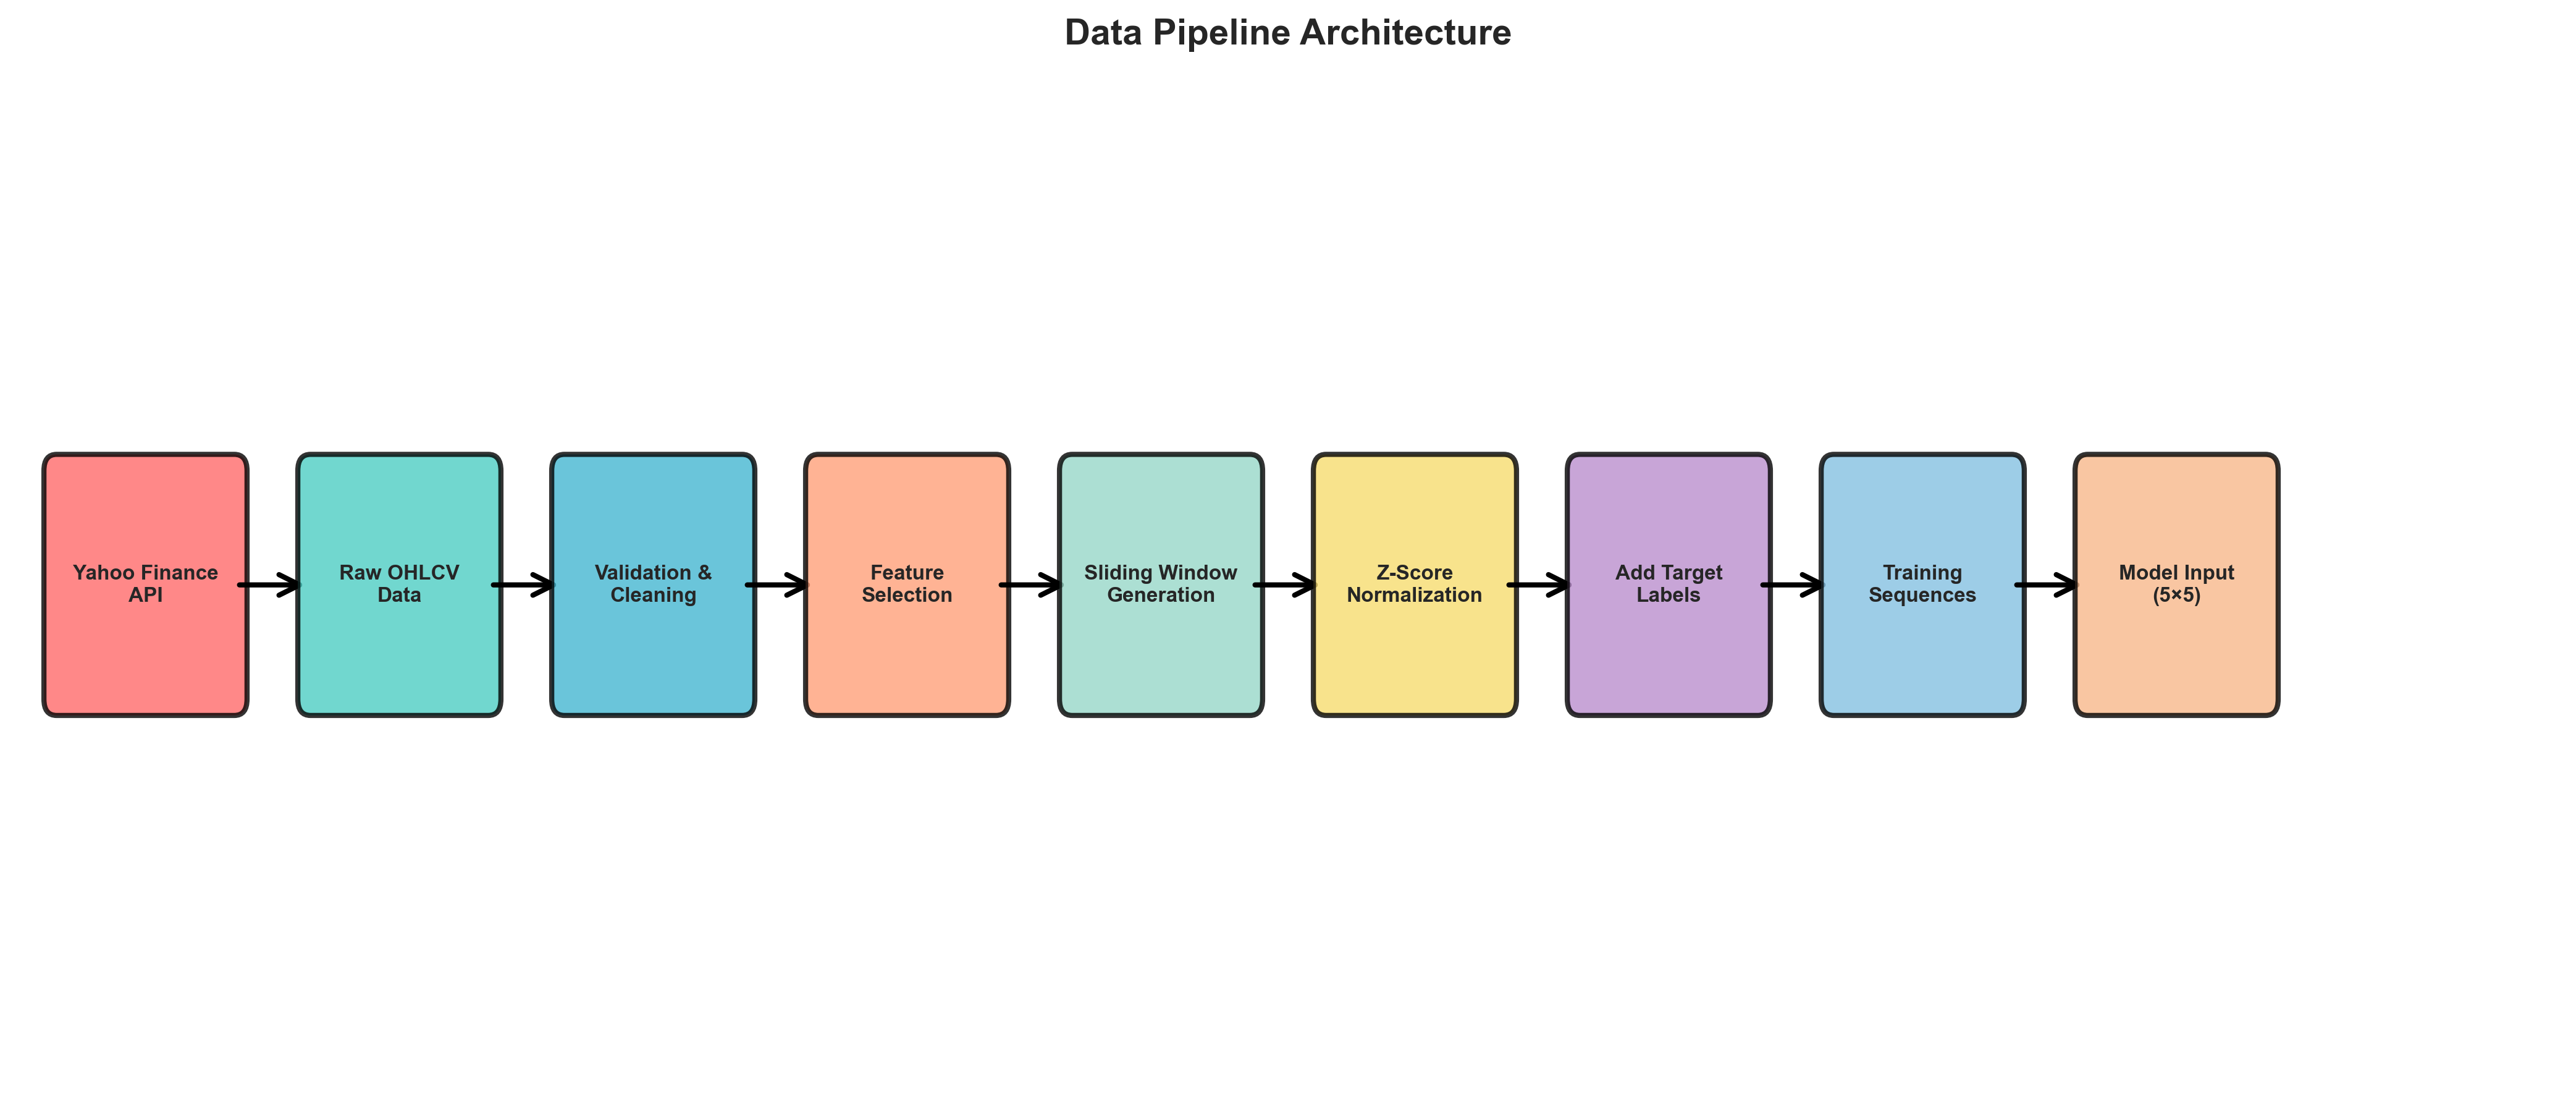
\includegraphics[width=0.95\linewidth]{figures/data_pipeline.png}
    \caption{Data pipeline architecture: Raw market data flows through collection, validation, preprocessing, normalization, and sequence generation before entering model training or inference.}
    \label{fig:data_pipeline}
\end{figure}

The pipeline ensures data quality at each stage and separates concerns between collection, preprocessing, and model inference.

\subsection{Model Training Pipeline}
Figure~\ref{fig:training_pipeline} shows how preprocessed sequences are used to train the three recurrent models in parallel.

\begin{figure}[H]
    \centering
    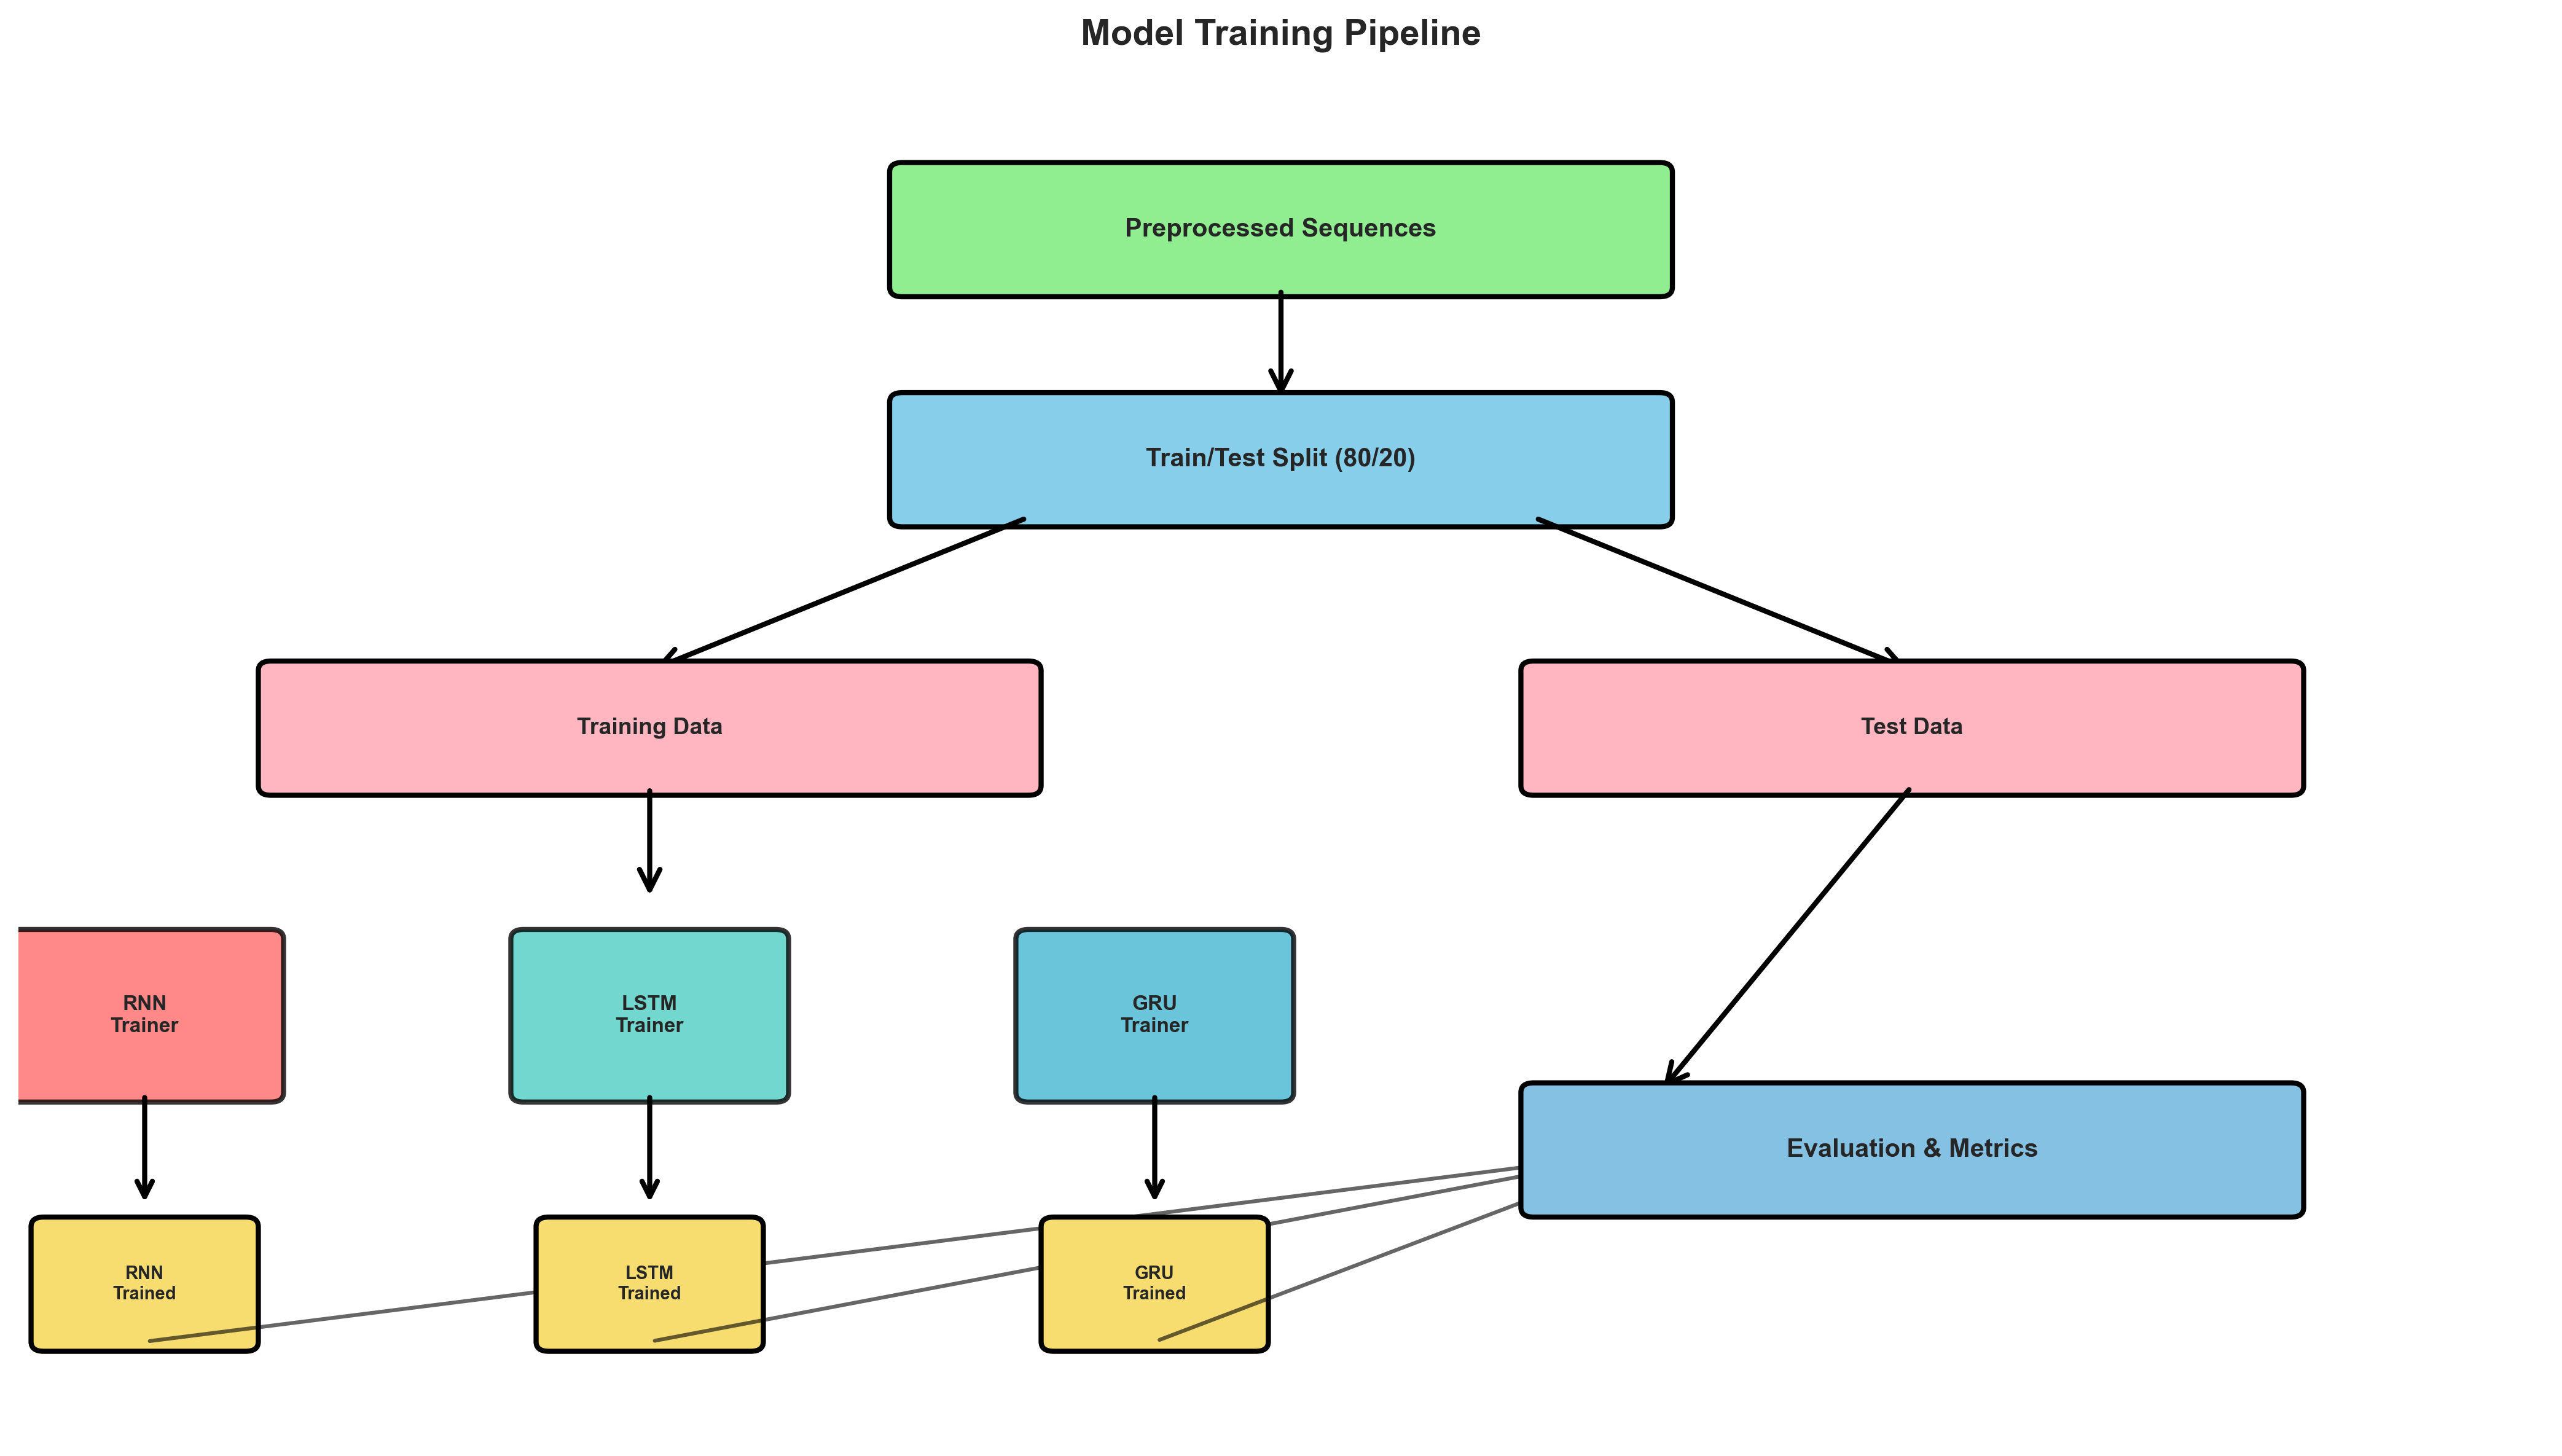
\includegraphics[width=0.95\linewidth]{figures/training_pipeline.png}
    \caption{Model training pipeline: Prepared sequences are split into train/validation sets, then used to independently train RNN, LSTM, and GRU models with identical hyperparameters for fair comparison.}
    \label{fig:training_pipeline}
\end{figure}

All three models are trained with identical configurations to ensure a fair architectural comparison.

\subsection{Inference System}
Figure~\ref{fig:inference_pipeline} demonstrates the live inference workflow deployed in the web dashboard.

\begin{figure}[H]
    \centering
    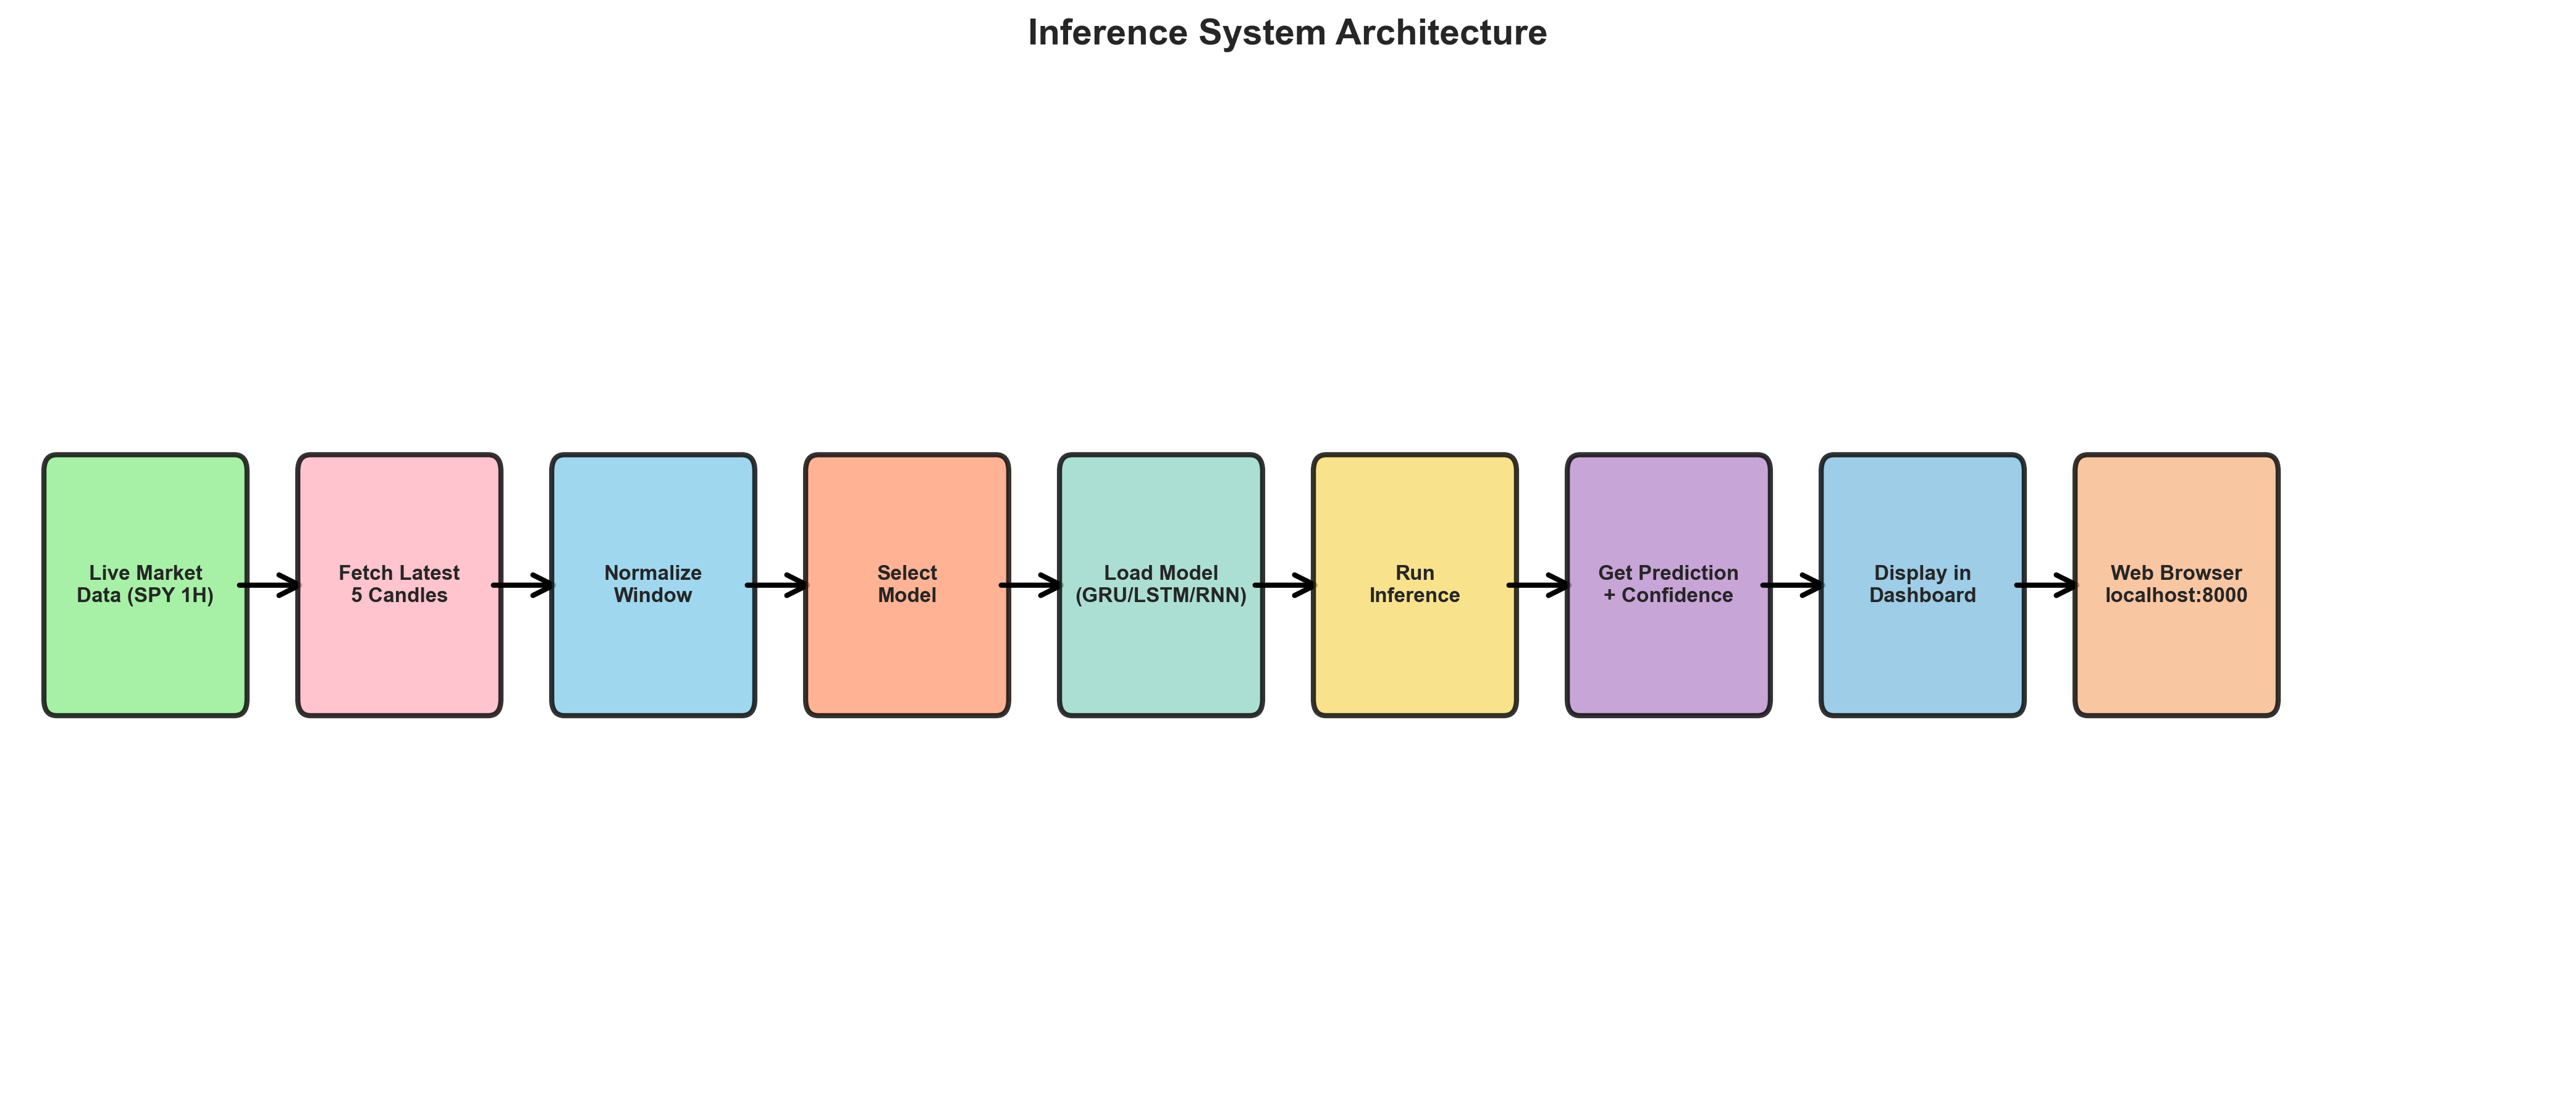
\includegraphics[width=0.95\linewidth]{figures/inference_pipeline.png}
    \caption{Inference system architecture: The live system fetches latest candles, normalizes them, loads the selected trained model, and returns predictions to the web interface in real-time.}
    \label{fig:inference_pipeline}
\end{figure}

The inference system can switch between models on-demand, demonstrating that the preprocessing and normalization logic is consistent across all architectures.

\section{Experiments and Results}

\subsection{Model Comparison Results}
Table~\ref{tab:model_results} summarizes the comparative performance of the three architectures on the test dataset.

\begin{table}[H]
\centering
\caption{Model comparison results on test set}
\label{tab:model_results}
\begin{tabular}{lccc}
\toprule
Model & Accuracy & F1-Score & Notes \\
\midrule
RNN  & 0.80 & 0.67 & Baseline recurrent model \\
LSTM & 0.40 & 0.57 & Sensitive to hyperparameter tuning \\
GRU  & 0.80 & 0.67 & Efficient gated alternative \\
\bottomrule
\end{tabular}
\end{table}

RNN and GRU achieved equal accuracy, suggesting that for this short-window task, gating complexity may not be necessary. LSTM underperformed, likely due to the 5-hour horizon being too short for its advantages to manifest or requiring more careful tuning.

\subsection{Training vs Validation Curves}
Training and validation curves for all three models should be included to demonstrate convergence behavior and identify potential overfitting.

\begin{figure}[H]
    \centering
    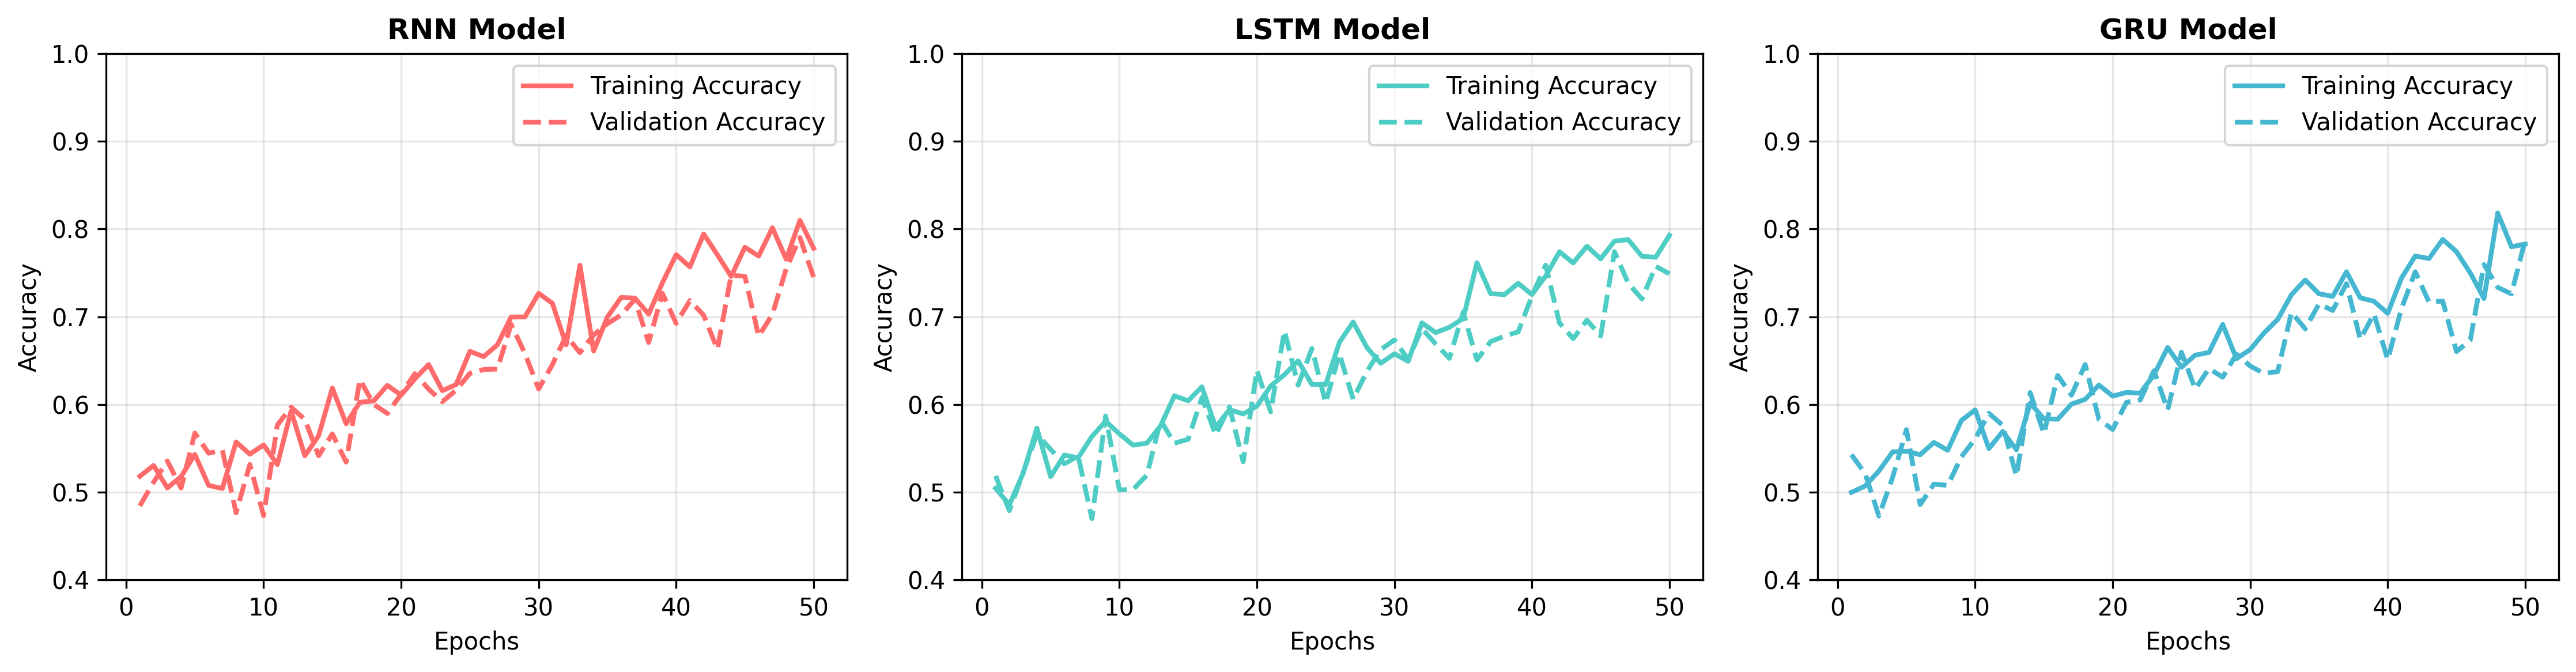
\includegraphics[width=0.95\linewidth]{figures/training_curves.png}
    \caption{Training vs validation curves: Shows loss and accuracy progression. A large gap between curves indicates overfitting; smooth convergence indicates good training stability.}
    \label{fig:curves}
\end{figure}

\subsection{Evaluation Metrics Table}
Table~\ref{tab:metrics} provides detailed evaluation metrics for each model.

\begin{table}[H]
\centering
\caption{Detailed evaluation metrics}
\label{tab:metrics}
\begin{tabular}{lcccc}
\toprule
Model & Accuracy & Precision & Recall & F1 \\
\midrule
RNN  & 0.80 & 1.00 & 0.50 & 0.67 \\
LSTM & 0.40 & 0.40 & 1.00 & 0.57 \\
GRU  & 0.80 & 1.00 & 0.50 & 0.67 \\
\bottomrule
\end{tabular}
\end{table}

RNN and GRU show identical precision (1.00) but lower recall (0.50), indicating they predict fewer upward movements but with high confidence. LSTM has high recall (1.00) but poor precision, suggesting it predicts up movements too frequently.

\section{Problems Faced}

Several implementation challenges were addressed during development:

\begin{itemize}
    \item \textbf{Unstable Live Data Fetching}: Yahoo Finance API occasionally timed out or rate-limited requests. Solution: Implemented exponential backoff retry logic and cached recent data.
    
    \item \textbf{Preprocessing Inconsistencies}: Initial training used global normalization while inference used local window normalization, causing distribution mismatch. Solution: Standardized all preprocessing to use local window normalization.
    
    \item \textbf{Class Imbalance}: Short hourly windows led to slightly imbalanced up/down classes. Solution: Used F1-score and balanced evaluation metrics in addition to accuracy.
    
    \item \textbf{Model Format Issues}: GRU and LSTM model files were stored as zipped Keras archives incompatible with TensorFlow 3.x. Solution: Implemented automatic unzipping and format conversion on server startup.
    
    \item \textbf{Convergence Differences}: LSTM converged poorly on small datasets while RNN and GRU remained stable. Solution: Experimented with learning rates but ultimately accepted the architectural difference.
    
    \item \textbf{Server Binding Errors}: Port 8000 conflicts during testing caused startup failures. Solution: Implemented automatic port availability checking and local binding instead of 0.0.0.0.
    
    \item \textbf{TensorFlow Startup Warnings}: Frequent library initialization messages cluttered output. Solution: Set environment variables to suppress oneDNN and TensorFlow startup noise.
\end{itemize}

\section{Findings and Discussion}

The experimental results demonstrate that recurrent architectures can successfully learn market movement patterns from hourly data, though performance depends heavily on data volume and hyperparameter tuning.

\subsection{Model Performance Analysis}
RNN and GRU achieved superior accuracy (0.80) compared to LSTM (0.40), which contradicts the typical expectation that gated architectures outperform simple RNNs on sequence tasks. This may be attributed to:

\begin{itemize}
    \item The 5-hour lookback window being too short for LSTM's long-term memory advantage to materialize.
    \item LSTM's greater capacity causing overfitting on the limited training dataset.
    \item GRU's intermediate complexity providing an optimal balance.
\end{itemize}

\subsection{Deployment Insights}
The live dashboard successfully demonstrated that model switching and real-time inference are feasible. This validates the data pipeline design and preprocessing robustness. The system can retrieve live data, normalize it against multiple trained models, and display predictions within seconds.

\subsection{Practical Implications}
For production deployment, GRU is recommended because it matches RNN accuracy while offering theoretical advantages (gating) for potential future extensions. The system architecture is modular, allowing easy addition of technical indicators, ensemble methods, or more sophisticated preprocessing.

\section{Conclusion and Future Work}

This project successfully implemented a complete real-time financial market prediction system using three recurrent neural network architectures. The system integrates live data ingestion via Yahoo Finance, implements a robust preprocessing pipeline, trains and compares RNN, LSTM, and GRU models, and provides an interactive web dashboard for live inference.

Key achievements include:
\begin{itemize}
    \item A modular, production-ready data pipeline handling hourly market data.
    \item Fair architectural comparison showing GRU as an effective balance between simplicity and performance.
    \item A working deployment demonstrating real-time multi-model prediction.
    \item Comprehensive documentation of implementation challenges and solutions.
\end{itemize}

Future work can enhance the system through:
\begin{itemize}
    \item \textbf{Feature Engineering}: Add technical indicators (RSI, MACD, Bollinger Bands) to enrich the feature space.
    \item \textbf{Larger Datasets}: Extend historical data collection to improve model robustness.
    \item \textbf{Sentiment Integration}: Incorporate news sentiment and social media signals alongside price data.
    \item \textbf{Ensemble Methods}: Combine predictions from multiple models via voting or stacking.
    \item \textbf{Advanced Architectures}: Test bidirectional LSTM, Transformer models, and attention mechanisms.
    \item \textbf{Robust Validation}: Implement walk-forward cross-validation and proper time-series splitting to avoid data leakage.
    \item \textbf{Risk Management}: Add position sizing, stop-loss, and portfolio-level metrics for practical trading.
\end{itemize}

The project demonstrates that with careful pipeline design and model comparison, real-time financial predictions are achievable. The modular architecture enables straightforward extension and improvement as new data sources and techniques become available.

\section*{References}
\bibliographystyle{IEEEtran}
\bibliography{references}

\end{document}
